\chapter{Theoretical Background}

In this chapter, we delve into the theoretical foundations that underpin the development and implementation of the Cartoonizer project. Specifically, we explore the \textbf{K-means algorithm}, a core clustering technique employed for data partitioning, and its critical role in \textbf{color quantization}, a process that simplifies the color representation of images. 

The K-means algorithm is essential for grouping image pixels based on their color properties, enabling efficient clustering and compression of color information. By leveraging this technique, we achieve the desired artistic effect of cartoonization through reduced and simplified color palettes. The subsequent sections provide a detailed overview of these concepts, discussing their principles, challenges, and applications, and laying the groundwork for the project's computational and visual objectives.

\section{K-Means algorithm}
K-means clustering is a fundamental algorithm in unsupervised machine learning, widely employed for partitioning a dataset into a predefined number of clusters, \( K \), based on feature similarity. The algorithm is iterative and aims to minimize the variance within each cluster, leading to compact and well-separated groups of data points.
The K-means algorithm operates by alternating between assignment and update steps until convergence. The process can be described as follows:

\begin{enumerate}
    \item \textbf{Initialization}: Select \( K \) initial centroids randomly from the dataset.
    \item \textbf{Assignment Step}: Assign each data point to the nearest centroid using a distance metric, commonly the Euclidean distance.
    \item \textbf{Update Step}: Calculate the new centroids by taking the mean of all data points assigned to each cluster.
    \item \textbf{Convergence}: Repeat the assignment and update steps until the centroids stabilize, or a maximum number of iterations is reached.
\end{enumerate}


The objective of K-means is to minimize the sum of squared distances between each data point and the centroid of its assigned cluster. Mathematically, this is represented as:

\[
J = \sum_{i=1}^{n} \sum_{k=1}^{K} \mathbf{1}(y_i = k) \|\mathbf{x_i} - \mu_k\|^2
\]

Where:
\begin{itemize}
    \item \( J \): The within-cluster sum of squared distances (WCSSD).
    \item \( \mathbf{x_i} \): The \( i \)-th data point.
    \item \( \mu_k \): The centroid of the \( k \)-th cluster.
    \item \( \mathbf{1}(y_i = k) \): An indicator function that equals 1 if data point \( \mathbf{x_i} \) is assigned to cluster \( k \), and 0 otherwise.
\end{itemize}

The algorithm alternates between minimizing \( J \) by assigning data points to their closest centroids and recalculating centroids based on these assignments.

\begin{figure}[H]
    \centering
    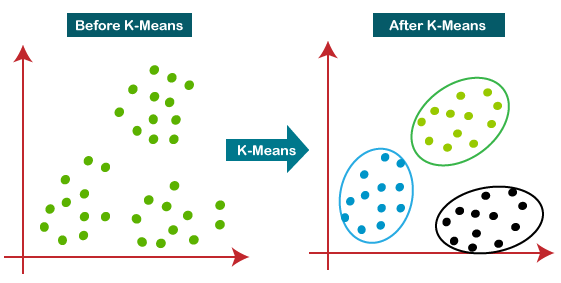
\includegraphics[width=0.7\textwidth]{images/kmeans.png}
    \caption{Set of data before and after the application of the K-Means algorithm}
    \label{fig:k_means}
\end{figure}


\subsection{Advantages and Limitations}
K-means is valued for its simplicity, efficiency, and scalability:
\begin{itemize}
    \item \textbf{Simplicity}: Easy to implement and interpret.
    \item \textbf{Efficiency}: Computationally efficient for moderate values of \( K \) and large datasets.
    \item \textbf{Versatility}: Applicable to a wide range of domains, including image compression and customer segmentation.
\end{itemize}


Despite its strengths, K-means has several limitations:
\begin{itemize}
    \item \textbf{Choice of \( K \)}: Requires prior knowledge of the number of clusters.
    \item \textbf{Initialization Sensitivity}: Poor initialization can lead to suboptimal clustering.
    \item \textbf{Cluster Shape Assumption}: Assumes clusters are spherical and of equal size, which may not hold for all datasets.
    \item \textbf{Outliers}: Sensitive to outliers, which can distort cluster centroids.
\end{itemize}

\subsection{Applications}

K-means clustering has numerous applications, including:
\begin{itemize}
    \item \textbf{Image Processing}: Color quantization and compression by reducing the number of colors in an image.
    \item \textbf{Market Segmentation}: Grouping customers based on purchasing behavior for targeted marketing.
    \item \textbf{Data Summarization}: Simplifying datasets by grouping similar data points.
    \item \textbf{Anomaly Detection}: Identifying outliers as data points that do not fit into any cluster well.
\end{itemize}

\subsection{Conclusion}

K-means clustering remains a foundational algorithm in machine learning due to its simplicity and effectiveness in solving clustering problems. While it has limitations, various extensions and initialization strategies, such as K-means++, have been developed to address these issues and improve the algorithm's robustness.


\section{Color Quantization}

Color quantization is a process used in image processing to reduce the number of distinct colors in an image while preserving its visual quality as much as possible. This is achieved by mapping the colors of the image to a smaller set of representative colors, known as a color palette. The result is a compressed image that retains its key visual features while using fewer colors.

\subsection{Purpose and Applications}

The main purpose of color quantization is to optimize image storage, processing, and transmission by reducing the complexity of the color information. It is widely used in several fields, including:

\begin{itemize}
    \item \textbf{Image Compression}: Reducing storage requirements for digital images by representing them with fewer colors.
    \item \textbf{Computer Graphics}: Rendering images efficiently on devices with limited color display capabilities.
    \item \textbf{Printing}: Mapping colors to a specific printer color gamut to ensure accurate reproduction.
    \item \textbf{Artistic Filters}: Creating stylized effects, such as cartoonization or posterization, by limiting the number of colors.
\end{itemize}

\subsection{Quantization Process}

The process of color quantization typically involves the following steps:

\begin{enumerate}
    \item \textbf{Color Space Selection}: Choose a color space (e.g., RGB, HSV, or CIE-Lab) for representing the image's pixel values. The choice of color space can influence the effectiveness of quantization, as some spaces better capture perceptual differences between colors.
    
    \item \textbf{Clustering of Colors}: Group similar colors into clusters. Each cluster represents a single color in the reduced palette. Clustering algorithms, such as K-means, are commonly used for this purpose. The goal is to minimize the perceptual difference between the original image and the quantized image.
    
    \item \textbf{Color Mapping}: Replace the original colors of the image with the nearest colors from the reduced palette. This step assigns each pixel in the image to the color of its cluster centroid.
\end{enumerate}

\begin{figure}[H]
    \centering
    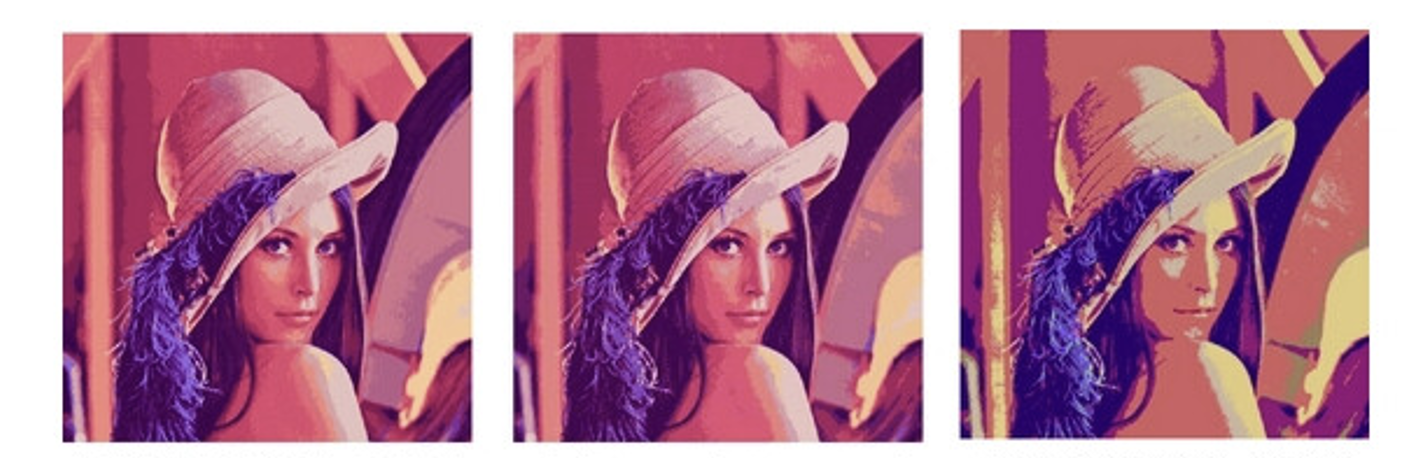
\includegraphics[width=0.7\textwidth]{images/color_quantization.png}
    \caption{Different color quantization algorithms applied to the same image}
    \label{fig:color_quantization}
\end{figure}

\subsection{Challenges in Color Quantization}

Color quantization is not without its challenges, which include:

\begin{itemize}
    \item \textbf{Perceptual Quality}: Reducing the number of colors can lead to visible artifacts or loss of detail, especially in images with subtle gradients.
    \item \textbf{Optimal Palette Selection}: Determining the optimal number and placement of colors in the palette is critical for balancing compression and visual fidelity.
    \item \textbf{Computational Cost}: Algorithms like K-means can be computationally expensive for high-resolution images, particularly with a large number of clusters.
    \item \textbf{Handling Outliers}: Outlier colors that do not belong to any major cluster can significantly affect the quality of the quantized image.
\end{itemize}


\subsection{Conclusion}

Color quantization is a crucial step in many image processing applications, balancing the trade-off between reducing storage requirements and maintaining visual quality. Techniques such as K-means clustering and median cut have been instrumental in achieving effective quantization, though challenges remain in optimizing perceptual quality and computational efficiency. In this work, color quantization plays a key role in achieving the desired cartoon-style effect by reducing the complexity of the image while preserving its essential features.

